\rule{0.5\textwidth}{0.5pt}\\

	{\large \textbf{EXPERIMENT NewEncConv80000-1}}\\
	
	{\normalsize HYPERPARAMETERS:}
	\begin{lstlisting}	
	*ARCHITECTURE HYPERPARAMETERS:
		-Encoder + Convolutional
		-Convolutional Layers: [1024, 512, 256, 256]
		-Convolutonal Kernels: [(3, 3), (3, 3), (3, 3), (3, 3)]
		-Convolutional Activation: relu
		-Output Layer Activation: linear
	
	*COMPILATION HYPERPARAMETERS:
		-Optimizer: ADAM lr=0.0001, beta_1=0.9, beta_2=0.999
		-Loss Function: MSE
		-Metric: MSE
	
	* TRAINING HYPERPARAMETERS:
		-Epochs: 100
		-Batch size: 32
		-Callbacks:
			-ReduceLROnPlateau: MSE 8 x0.1
			-Early Stop: MSE 15
	\end{lstlisting}
	
	{\normalsize VISUALIZATION:}
	\begin{lstlisting}
	*RESULTS:
        -Train MSE: 0.0163
        -Validation MSE: 0.0369
	\end{lstlisting}
	
	\begin{figure*}[ht!]
		\subfloat[IGNORE THIS EVOLUTION FIGURE, TRAINING FINISHED BEFORE STORING THE HISTORY, THIS IS FROM THE PREVIOUS EXPERIMENT]{%
		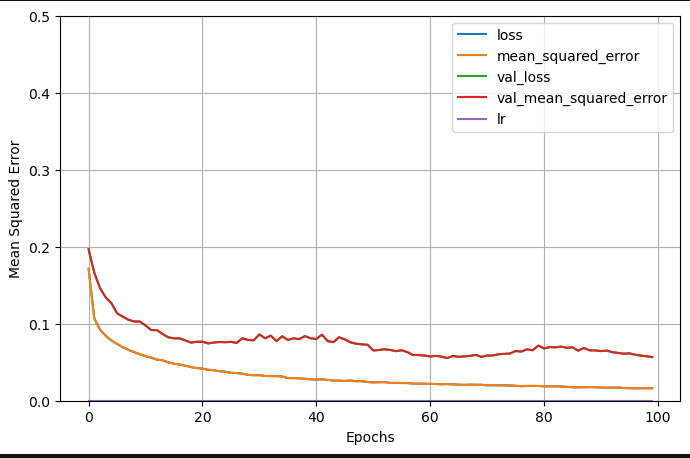
\includegraphics[ width=0.31\textwidth]{ap-NewEncConv30000-1-evolution.png}}
		\hspace{\fill}
		\subfloat[Validation example]{%
		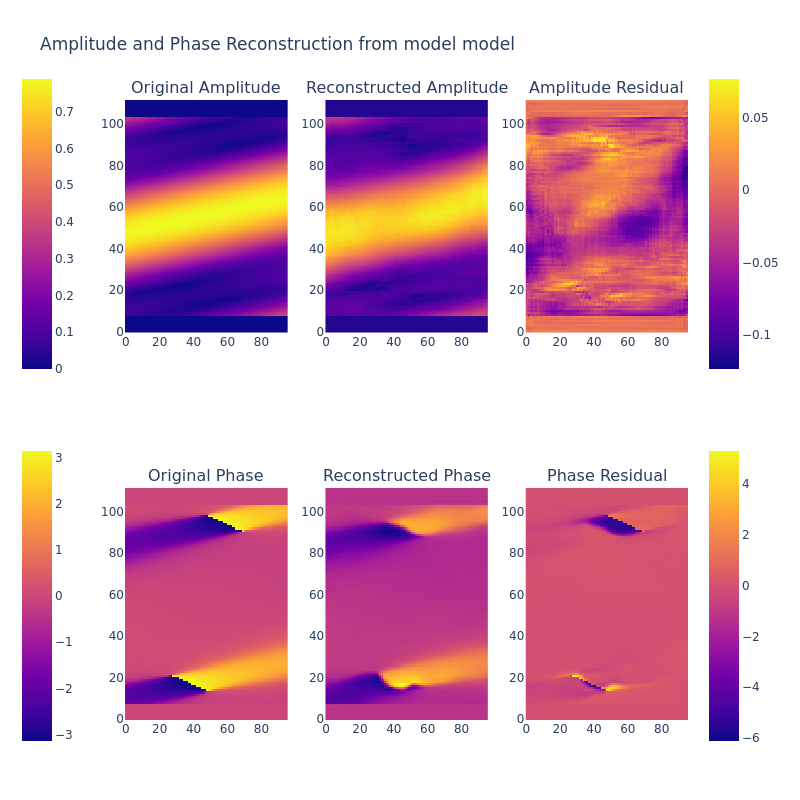
\includegraphics[ width=0.31\textwidth]{ap-NewEncConv80000-1-val.png}}
		\hspace{\fill}
		\subfloat[Train example]{%
		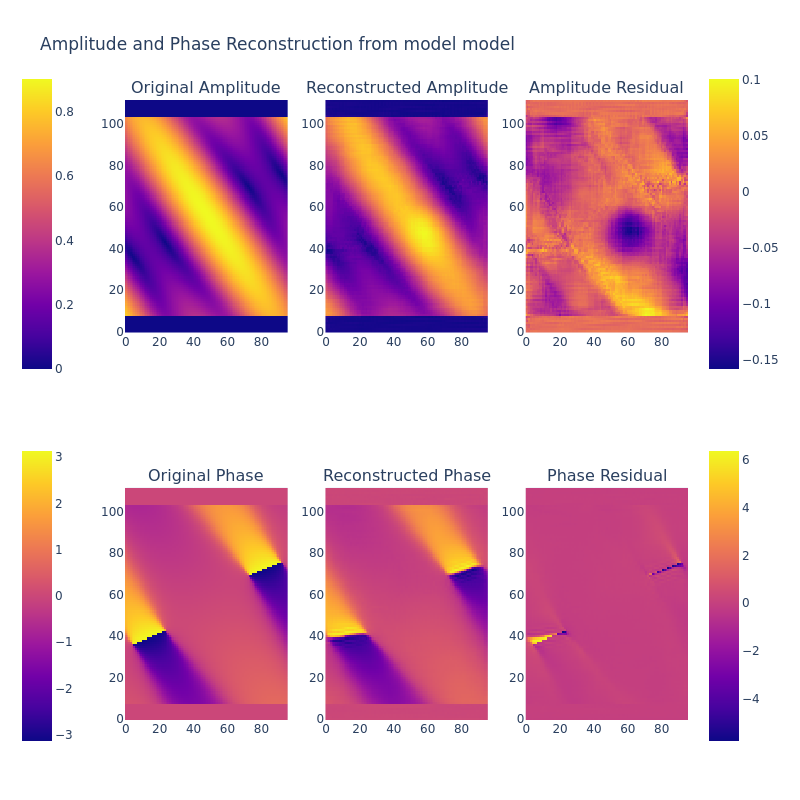
\includegraphics[ width=0.31\textwidth]{ap-NewEncConv80000-1-train.png}}\\
		\caption{Results of training the model NewEncConv80000-1}
	\end{figure*}
	
\FloatBarrier	
\rule{0.5\textwidth}{0.5pt}\\